\documentclass[border=6pt]{standalone}
% ---------------------------------------------------------------------------
% tikzpreamble.tex -- shared by main.tex and by every standalone in tikz/
% ---------------------------------------------------------------------------
\usepackage{amsmath}
\usepackage{amssymb}
\usepackage{tikz}
\usepackage{circuitikz}
\usetikzlibrary{arrows.meta,calc,positioning,decorations.pathmorphing,decorations.pathreplacing,
                decorations.markings,patterns,angles,quotes,fit,
                shapes.geometric,shapes.misc,backgrounds,intersections}

\ctikzset{bipoles/length=0.85cm}
\ctikzset{resistors/scale=0.85}
\ctikzset{capacitors/scale=0.9}

\tikzset{
  wire/.style      = {line width=0.7pt},
  dashedwire/.style= {line width=0.7pt, densely dashed},
  term/.style      = {circle, draw, line width=0.6pt, fill=white,
                      inner sep=0pt, minimum size=4.5pt},
  node dot/.style  = {circle, fill=black, inner sep=0pt, minimum size=4pt},
  boxlabel/.style  = {font=\sffamily\small},
  annot/.style     = {font=\small, align=left},
  phasor/.style    = {-{Stealth[length=3.2mm,width=2.2mm]}, line width=1.1pt},
  thinphasor/.style= {-{Stealth[length=2.6mm,width=1.8mm]}, line width=0.7pt},
  axis line/.style = {-{Stealth[length=2.6mm,width=1.8mm]}, line width=0.6pt},
  guide/.style     = {densely dashed, line width=0.4pt, gray},
}
\usepackage{siunitx}

\begin{document}
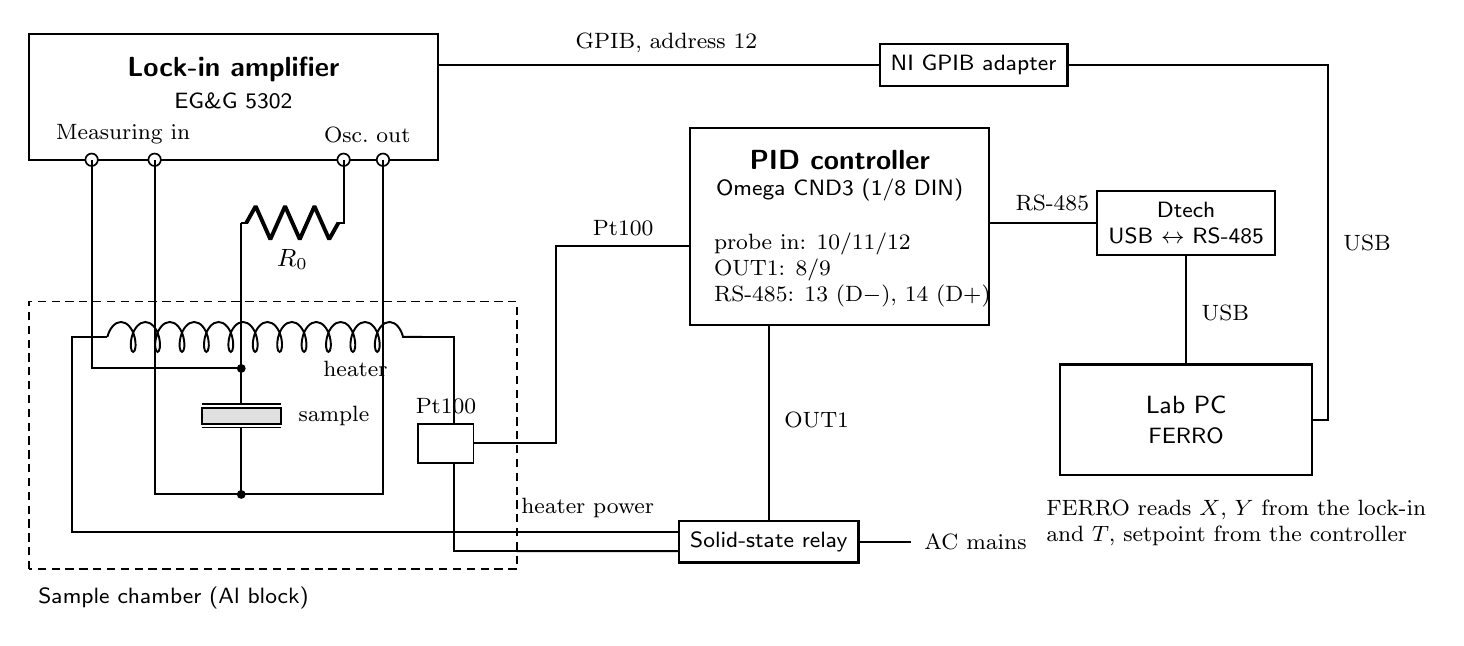
\begin{tikzpicture}[
    every node/.style={font=\small},
    instr/.style   = {draw, line width=0.8pt, align=center,
                      font=\sffamily\small, inner sep=5pt},
    small instr/.style = {draw, line width=0.8pt, align=center,
                      font=\sffamily\footnotesize, inner sep=4pt},
    lead/.style    = {font=\footnotesize, inner sep=2pt},
  ]

  % =======================================================================
  %  Lock-in amplifier and the measuring circuit
  % =======================================================================
  \draw[wire] (0.2,5.4) rectangle (5.4,7.0);
  \node[boxlabel,font=\sffamily\bfseries] at (2.8,6.55) {Lock-in amplifier};
  \node[boxlabel,font=\sffamily\footnotesize] at (2.8,6.15) {EG\&G 5302};
  \node[boxlabel,font=\footnotesize] at (1.4,5.72) {Measuring in};
  \node[boxlabel,font=\footnotesize] at (4.5,5.72) {Osc.\ out};
  \foreach \x in {1.0,1.8,4.2,4.7} { \node[term] at (\x,5.4) {}; }

  % ---- sample chamber ----------------------------------------------------
  \draw[dashedwire] (0.2,0.2) rectangle (6.4,3.6);
  \node[boxlabel,font=\sffamily\footnotesize,anchor=north west] at (0.2,0.10)
        {Sample chamber (Al block)};

  % heater winding, with both leads taken out at the bottom right
  \draw[wire,decorate,decoration={coil,aspect=0.5,segment length=3.1mm,amplitude=1.9mm}]
        (1.2,3.15) -- (5.2,3.15);
  \node[lead,anchor=north] at (4.35,2.92) {heater};
  \draw[wire] (1.2,3.15) -- (0.75,3.15) -- (0.75,0.67) -- (6.4,0.67);
  \draw[wire] (5.2,3.15) -- (5.6,3.15) -- (5.6,0.43) -- (6.4,0.43);

  % sample capacitor
  \draw[wire] (2.4,2.30) -- (3.4,2.30);
  \draw[wire,fill=black!12] (2.4,2.05) rectangle (3.4,2.25);
  \draw[wire] (2.4,2.00) -- (3.4,2.00);
  \draw[wire] (2.9,2.30) -- (2.9,4.60);
  \draw[wire] (2.9,2.00) -- (2.9,1.15);
  \node[lead,anchor=west] at (3.55,2.15) {sample};

  % Pt100 probe in the block
  \draw[wire,fill=white] (5.15,1.55) rectangle (5.85,2.05);
  \node[lead,anchor=south] at (5.5,2.10) {Pt100};
  \draw[wire] (5.85,1.80) -- (6.4,1.80);

  % drive branch through R0, the return, and the measuring leads
  \draw[wire] (4.2,5.4) -- (4.2,4.60) to[R=$R_0$] (2.9,4.60);
  \draw[wire] (4.7,5.4) -- (4.7,1.15) -- (2.9,1.15);
  \draw[wire] (1.0,5.4) -- (1.0,2.75) -- (2.9,2.75);
  \draw[wire] (1.8,5.4) -- (1.8,1.15) -- (2.9,1.15);
  \node[node dot,minimum size=3.2pt] at (2.9,2.75) {};
  \node[node dot,minimum size=3.2pt] at (2.9,1.15) {};

  % =======================================================================
  %  Temperature control
  % =======================================================================
  \draw[wire] (8.6,3.3) rectangle (12.4,5.8);
  \node[boxlabel,font=\sffamily\bfseries] at (10.5,5.40) {PID controller};
  \node[boxlabel,font=\sffamily\footnotesize] at (10.5,5.02) {Omega CND3 (1/8 DIN)};
  \node[boxlabel,font=\footnotesize,align=left,anchor=north west] at (8.78,4.60)
        {probe in: 10/11/12\\
         OUT1: 8/9\\
         RS-485: 13 (D$-$), 14 (D$+$)};

  \node[small instr] (ssr) at (9.6,0.55) {Solid-state relay};

  % Pt100 -> controller input
  \draw[wire] (6.4,1.80) -- (6.9,1.80) -- (6.9,4.30) -- (8.6,4.30);
  \node[lead,anchor=south] at (7.75,4.36) {Pt100};

  % heater -> relay (straight into the left-hand side of the relay)
  \draw[wire] (6.4,0.67) -- ($(ssr.west)+(0,0.12)$);
  \draw[wire] (6.4,0.43) -- ($(ssr.west)-(0,0.12)$);
  \node[lead,anchor=south] at (7.3,0.78) {heater power};

  % controller OUT1 -> relay control
  \draw[wire] (9.6,3.3) -- (ssr.north);
  \node[lead,anchor=west] at (9.72,2.10) {OUT1};

  % mains into the relay
  \draw[wire] (ssr.east) -- (11.4,0.55);
  \node[lead,anchor=west] at (11.5,0.55) {AC mains};

  % =======================================================================
  %  Computer links
  % =======================================================================
  \node[instr,minimum width=3.2cm,minimum height=1.4cm] (pc) at (14.9,2.10)
        {Lab PC\\ \footnotesize FERRO};
  \node[small instr] (dtech) at (14.9,4.60) {Dtech\\USB $\leftrightarrow$ RS-485};
  \node[small instr] (gpib)  at (12.2,6.60) {NI GPIB adapter};

  % RS-485 from the controller, USB to the PC
  \draw[wire] (12.4,4.60) -- (dtech.west);
  \node[lead,anchor=south] at (13.2,4.68) {RS-485};
  \draw[wire] (dtech.south) -- (pc.north);
  \node[lead,anchor=west] at (15.02,3.45) {USB};

  % GPIB from the lock-in
  \draw[wire] (5.4,6.60) -- (gpib.west);
  \node[lead,anchor=south] at (8.3,6.68) {GPIB, address 12};
  \draw[wire] (gpib.east) -- (16.7,6.60) -- (16.7,2.10) -- (pc.east);
  \node[lead,anchor=west] at (16.82,4.35) {USB};

  % what travels over each link
  \node[annot,font=\footnotesize,anchor=north west] at (13.0,1.20)
        {FERRO reads $X$, $Y$ from the lock-in\\
         and $T$, setpoint from the controller};
\end{tikzpicture}
\end{document}
